Die Systemarchitektur von \textit{LearnHub} schafft die technische Grundlage für eine gut 
wartbare und zukunftssichere Webplattform. Sie verfolgt das Ziel, die verschiedenen 
Funktionsbereiche – das Content-Management-System
sowie den Maturatrainer des Partnerprojekts – logisch voneinander abzugrenzen, 
ohne dabei deren effiziente Zusammenarbeit zu beeinträchtigen.

Zur Realisierung dieser Anforderungen wurde eine mehrschichtige Client-Server-Architektur implementiert.
Diese gewährleistet eine präzise Separation von Präsentation,
Logik und Datenverwaltung und bildet damit die Grundlage für wartungsfreundlichen
Betrieb und problemlose Systemerweiterungen.

\subsubsection{Architekturüberblick}
Die LearnHub-Plattform folgt einem klassischen Client-Server-Ansatz.
Das Frontend wird als benutzerinteraktive Schicht im Browser ausgeführt
und ist für die Präsentation der Oberfläche zuständig. 
Alle Anfrageverarbeitung, Geschäftslogik und Datenbankzugriffe erfolgen zentral im Backend.
Die Kommunikation zwischen Frontend und Backend läuft über REST-APIs auf Basis des HTTP-Protokolls ab.
Der Datenaustausch erfolgt im JSON-Format, was eine unkomplizierte Verarbeitung 
und optimale Interoperabilität sicherstellt.

Ein externes Authentifizierungs- und Autorisierungssystem bildet zusätzlich das Rückgrat 
für Benutzerverwaltung und rollenbasierte Zugriffskontrolle.

\begin{figure}[H]
    \centering
    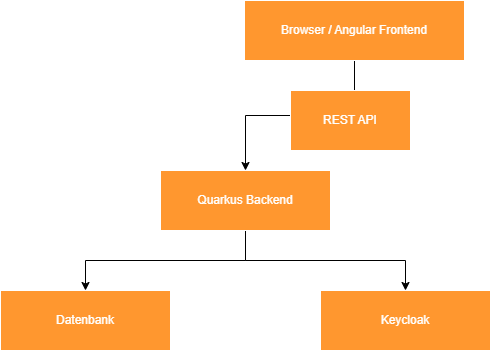
\includegraphics[width=0.85\textwidth]{pics/systemArchiktetur.png}
    \caption{Übersicht der Systemarchitektur von LearnHub}
    \label{fig:systemarchitektur}
\end{figure}

Abbildung~\ref{fig:systemarchitektur} zeigt eine Übersicht der Systemarchitektur
der LearnHub-Plattform und das Zusammenspiel der einzelnen Komponenten.

\subsubsection{Frontend-Architektur}

Das Frontend wurde mit Angular als Single-Page-Application (SPA) umgesetzt. 
Das ermöglicht ein flüssiges Nutzererlebnis, da Seitenwechsel ohne Neuladen der Seite erfolgen.
Das Frontend besteht aus mehreren Angular-Components, die jeweils für einen 
bestimmten Funktionsbereich zuständig sind, etwa den Fragenkonfigurator, den Maturaupload oder 
den persönlichen Bereich.
Die Logik und die Kommunikation mit dem Backend sind in sogenannten Services gekapselt. 
Diese Services kümmern sich um die HTTP-Anfragen zum Backend und liefern den Components die benötigten Daten.
Durch diese Aufteilung wird der Code wartbarer und lässt sich besser wiederverwenden.
Das Schema Separation of Concerns wird dadurch konsequent umgesetzt.
Für die Navigation verwendet das Frontend das Angular-Routing. 
Abhängig von der Rolle des angemeldeten Nutzers werden unterschiedliche Routen und 
Funktionalitäten freigeschaltet.

\subsubsection{Backend-Architektur}

Das Backend ist das Herzstück der Architektur und wurde mit Java und dem Framework Quarkus entwickelt. 
Es verarbeitet alle Anwendungslogik, prüft die Daten und verwaltet den Datenbankzugriff.

Das Backend ist in mehreren Schichten aufgeteilt:

\begin{itemize}
\item Boundary: REST-Endpunkte für die HTTP-Kommunikation mit dem Frontend
\item Model: Datenentitäten, die in der Datenbank gespeichert werden
\item Repository: Datenbankzugriff und Verwaltung der persistenten Daten
\item DTO (Data Transfer Object): Datenstrukturen für den Datentransfer zwischen Frontend und Backend
\item Mapper: Umwandlung zwischen Models und DTOs
\item Security: Integration mit Keycloak für Authentifizierung und Autorisierung sowie Berechtigungschecks
\end{itemize}

Alle Sicherheitsprüfungen laufen ausschließlich im Backend ab. 
Das stellt sicher, dass wichtige Sicherheitslogik nicht im Frontend umgesetzt wird.

\subsubsection{Authentifizierung und Autorisierung}

Die Anmeldung wird über Keycloak verwaltet, einen Identity-Provider, der von der 
Schule zur Verfügung gestellt wird. Keycloak nutzt moderne 
Sicherheitsstandards wie OAuth2.0.

Nach erfolgreicher Anmeldung erhält das Frontend ein JSON Web Token (JWT). 
Dieses Token enthält Informationen über die Rolle des Nutzers, also ob es sich um 
eine/n Schüler:in oder eine/n Lehrer:in handelt.
Das Token wird bei jeder Anfrage an das Backend mitgesendet, wo es überprüft wird.

Das Backend entscheidet basierend auf der Rolle aus dem Token, welche Ressourcen 
der/die Nutzer:in erreichen darf. Schüler:innen haben andere Berechtigungen als Lehrer:innen,
etwa beim Freigeben von Fragen, dem Verwalten von Fächern und Themenpools oder dem 
Bearbeiten öffentlicher Inhalte.

\subsubsection{Datenhaltung}

In dem Projekt wird eine relationale Datenbank verwendet, um alle relevanten Informationen zu speichern.
In der DB sind Benutzer, Fächer, Themenpools, Fragen, Mitschriften abgelegt.
Für die Entwicklung wird die In-Memory-Datenbank H2 verwendet, während für den Produktivbetrieb 
auf der VM MySQL zum Einsatz kommt.
Durch die strukturierte Datenverwaltung können Fragen und Unterlagen eindeutig 
einem Fach oder Themenpool zugeordnet werden. 
Das bildet die Grundlage für die Navigation in der Plattform und
ermöglicht den filterbasierten Lernmodus.

\subsubsection{Containerisierung und Deployment}

Frontend und Backend laufen in Docker-Containern auf einer VM der Schule.
Dort wird immer die aktuelle Version deployed.
Das bringt Vorteile: Die Umgebung ist überall gleich, die Anwendung lässt sich leicht 
reproduzieren und skalieren. Die Komponenten sind klar voneinander getrennt.